\documentclass[a4paper,12pt]{report}
\usepackage[utf8]{inputenc}
\usepackage[francais]{babel}
\usepackage[T1]{fontenc}
\usepackage{graphicx}
\usepackage{listingsutf8}
\usepackage[colorlinks,urlcolor=blue]{hyperref} %hyperlinks
\usepackage[nottoc,notlot,notlof]{tocbibind} %To bind the table of contents to the bibligoraphy
\usepackage{../../packages/tikz-uml} %UML elements

\begin{document}
%----------------------------------------------------------------------------------------
%   TITLE PAGE
%----------------------------------------------------------------------------------------
\begin{titlepage}
\newcommand{\HRule}{\rule{\linewidth}{0.5mm}} % Defines a new command for the horizontal lines
\center
%----------------------------------------------------------------------------------------
%   LOGOS SECTION
%----------------------------------------------------------------------------------------

\includegraphics[scale=0.5]{images/umLogo.png} % Université de Montpellier Logo
\hspace{\fill}

\includegraphics[scale=0.25]{images/fdsLogo.jpg} % Faculté de Sciences Logo
%----------------------------------------------------------------------------------------
%   HEADING SECTIONS
%----------------------------------------------------------------------------------------
\textsc{\LARGE M1 Informatique AIGLE}\\[1cm]
\textsc{\Large \textbf{HMIN122M}}\\[0.25cm]
\textsc{\large Mini-Projet : entrepôts de données}\\[0.8cm]
%----------------------------------------------------------------------------------------
%   TITLE SECTION
%----------------------------------------------------------------------------------------
\HRule \\[0.4cm]
{ \huge \bfseries Rendu sur la modélisation d'un entrepôts de données}\\[0.4cm]
\HRule \\[0.8cm]
%----------------------------------------------------------------------------------------
%   AUTHORS SECTION
%----------------------------------------------------------------------------------------
\begin{minipage}{\textwidth}
\centering \huge
Bachar \textsc{Rima}\\ % Student
Joseph \textsc{Saba}\\ % Student
Tasnim \textsc{Shaqura Muhammad}\\ % Student
Jérémy \textsc{Bourgin} % Student
\end{minipage} \\[0.8cm]
%----------------------------------------------------------------------------------------
%   DATE SECTION
%----------------------------------------------------------------------------------------
{\large 23 octobre 2018}\\[1cm]
\hspace{\fill}
\vfill % Fill the rest of the page with whitespace
\end{titlepage}

\pagestyle{plain}

{
  \hypersetup{linkcolor=black}
  \tableofcontents
}

\newpage

\chapter*{Introduction}
\label{chap:intro}
\addcontentsline{toc}{chapter}{\nameref{chap:intro}}
Dans le cadre du mini-projet du module \textbf{HMIN122M}, nous avons décidé de modéliser un entrepôts de données pour le réseau de transport publique de Montpellier, \textit{tam-voyages}. Pour ce faire, nous avons proposé des \textit{data marts} formant le \textit{data warehouse} et permettant de réaliser des requêtes analytiques sur un ensemble important de données. Cette modélisation permettra ainsi de mettre en \oe{}uvre un outil d'analyse permettant de bien répondre aux problématiques suivantes :
\begin{enumerate}
  \item Comment \textit{tam-voyages} pourront-ils augmenter leur taux de ventes en se basant sur la circulation du réseau\footnote{en particulier en examinant les lignes de tramway et les bus} ?
  \item Comment \textit{tam-voyages} pourront-ils suivre l'évolution et la maintenance de leurs matériaux de manière à réduire les dépenses qui y sont associées ?
\end{enumerate}

Ces problématiques seront ainsi adressées en analyzant les actions et opérations effectuées par \textit{tam-voyages}, notamment en choisissant celles qui paraissent les plus pertinentes et les plus importantes en termes de données intégrées et flexibilité des critères d'analyse.

\chapter*{Questions}
\label{chap:questions}
\addcontentsline{toc}{chapter}{\nameref{chap:questions}}

\section*{Question 1}
\label{sec:question_1}
\addcontentsline{toc}{section}{\nameref{sec:question_1}}

Les actions/opérations effectuées par \textit{tam-voyages} considérées :
\begin{itemize}
  \item Les voyages.
  \item La maintenance de véhicules.
  \item Les ventes de tickets et les abonnements.
  \item Les amendes.
\end{itemize}

\section*{Question 2}
\label{sec:question_2}
\addcontentsline{toc}{section}{\nameref{sec:question_2}}

\begin{enumerate}
  \item exemples de requêtes analytiques pour l'action \og voyages \fg :
  \begin{itemize}
    \item \texttt{le nombre de voyageurs par bus, utilisant des tickets pour le mois de juillet.}
    \item \texttt{le prix moyen par type de ticket pour chaque voyage pendant les vacances de noël de 2018.}
    \item \texttt{le nombre de voyageurs abonnés par ligne pour chaque voyage pour les deux derniers mois.}
    \item \texttt{l'arrêt le plus fréquenté par toutes les lignes de circulation.}
  \end{itemize}
  \item exemples de requêtes analytiques pour l'action \og maintenance \fg :
  \begin{itemize}
    \item \texttt{le nombre de bus maintenus pour le mois de septembre 2018.}
    \item \texttt{les X premières lignes ayant le nombre maximale de maintenances par mois.}
    \item \texttt{les X premières véhicules nécessitant le plus de maintenance pour les 6 dernier mois.}
  \end{itemize}
  \item exemples de requêtes analytiques pour l'action \og ventes \fg :
  \begin{itemize}
    \item \texttt{le nombre d'abonnés ayant plus que 26 ans pour le mois d'août 2018.}
    \item \texttt{le nombre d'abonnés par date de naissance pour l'année 2018.}
    \item \texttt{les types d'abonnement les plus fréquents pour l'année 2018.}
  \end{itemize}
  \item exemples de requêtes analytiques pour l'action \og amendes \fg :
  \begin{itemize}
    \item \texttt{les lignes qui ont générées le plus d'amendes pour les deux derniers mois.}
    \item \texttt{les lignes les plus contrôllées de la semaine dernière.}
    \item \texttt{le nombre des abonnés qui ont reçu des amendes par ligne, l'avant-midi.}
    \item \texttt{la somme total d'amendes rapportée par type de voyageur par ligne pour le dernier mois.}
  \end{itemize}
\end{enumerate}

\section*{Question 3}
\label{sec:question_3}
\addcontentsline{toc}{section}{\nameref{sec:question_3}}

Les actions considérées, par ordre d'importance:
\begin{enumerate}
  \item \og voyages \fg.
  \item \og ventes \fg.
  \item \og maintenance \fg.
  \item \og amendes \fg.
\end{enumerate}

\section*{Question 4}
\label{sec:question_4}
\addcontentsline{toc}{section}{\nameref{sec:question_4}}

Les actions les plus pertinentes à analyser vis-à-vis les problématiques avancées sont \og voyages \fg et \og maintenance \fg qu'on traitera de la manière suivante :
\begin{description}
  \item [voyages :] modèle en étoile détaillé.
  \item [maintenance :] modèle en étoile \textit{moins} détaillé, en particulier le modèle intitulé "\textit{periodic snapshot}".
\end{description}

\section*{Questions 5 et 6}
\label{sec:question_5_6}
\addcontentsline{toc}{section}{\nameref{sec:question_5_6}}

\subsection*{\textit{Data Mart} de \og voyages \fg}
\label{subsec:data_mart_voyages}
\addcontentsline{toc}{subsection}{\nameref{subsec:data_mart_voyages}}
\begin{figure}[!ht]
  \centering
  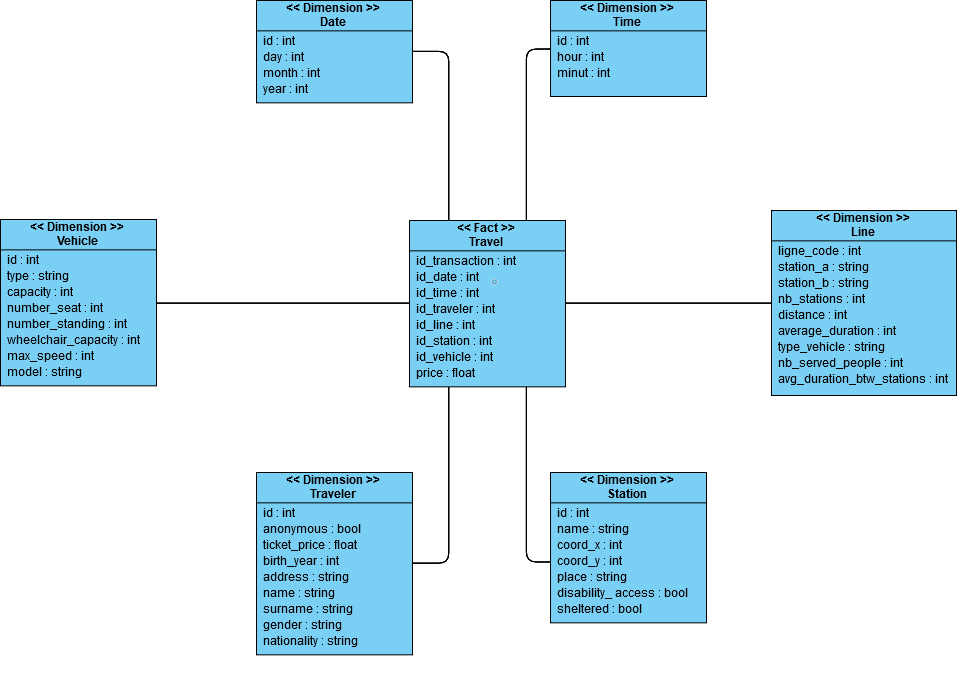
\includegraphics[scale=0.65]{images/voyages_datamart.png}
  \caption{modèle en étoile de l'action \og voyages \fg}
\end{figure}

Les mesures de la table des voyages sont :
\begin{itemize}
  \item \texttt{cost\_travel} : additive
\end{itemize}

\newpage

\subsection*{\textit{Data Mart} de \og maintenance \fg}
\label{subsec:data_mart_maintenance}
\addcontentsline{toc}{subsection}{\nameref{subsec:data_mart_maintenance}}
\begin{figure}[!ht]
  \centering
  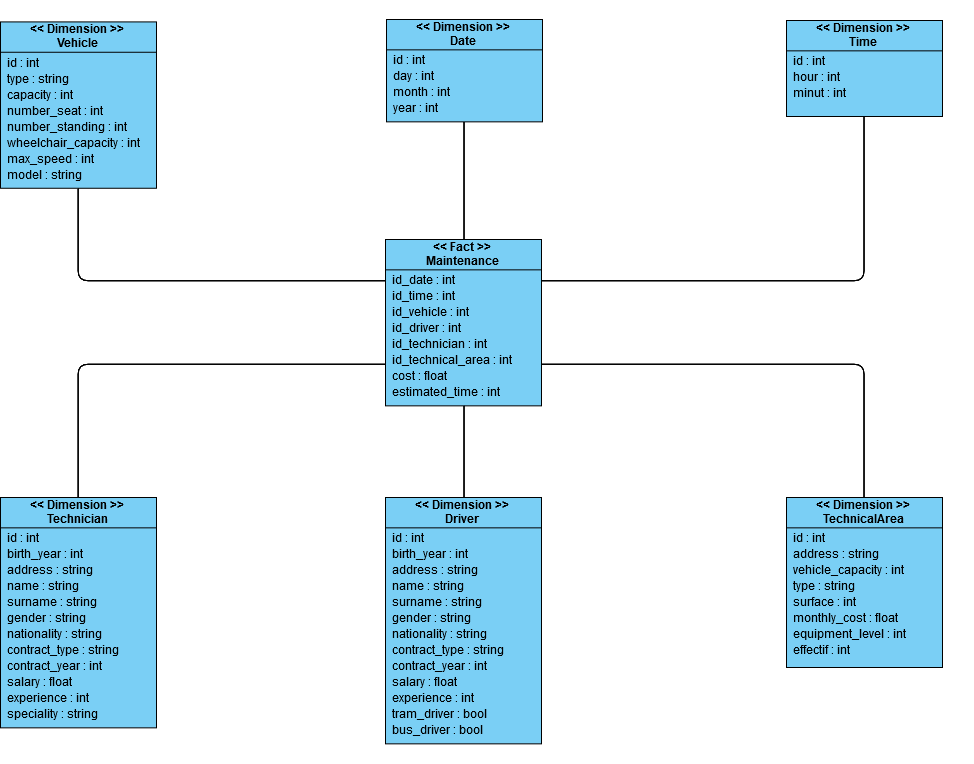
\includegraphics[scale=0.65]{images/maintenance_datamart.png}
  \caption{modèle en étoile de l'action \og maintenance \fg}
\end{figure}

Les mesures de la table des maintenances sont :
\begin{itemize}
  \item \texttt{cost} : additive
  \item \texttt{estimated\_time} : additive
\end{itemize}

\newpage

\subsection*{\textit{Data warehouse} de \textit{tam-voyages}}
\label{subsec:data_warehouse}
\addcontentsline{toc}{subsection}{\nameref{subsec:data_warehouse}}
\begin{figure}[!ht]
  \centering
  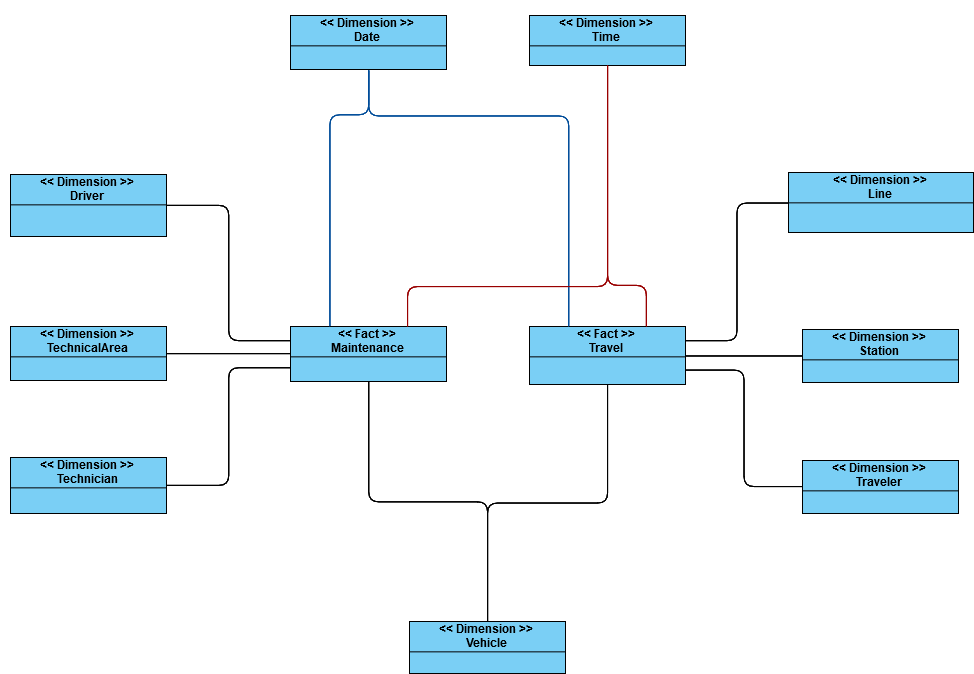
\includegraphics[scale=0.6]{images/data_warehouse.png}
  \caption{le \textit{data warehouse} résultant}
\end{figure}

\newpage

\subsubsection{Remarques}
\begin{itemize}
  \item l'attribut \textbf{id\_travel} de la table \texttt{Travel} est la clé primaire utilisé pour identifier un voyage (\textit{dimension dégénérée}).
  \item l'attribut \textbf{cost\_travel} de la table \texttt{Travel} désigne le coût du voyage.
  \item l'attribut \textbf{avg\_served\_people} de la table \texttt{Line} désigne le nombre de passagers en moyenne désservis par la ligne.
  \item l'attribut \textbf{place} de la table \texttt{Station} désigne l'endroit où se trouve la station (avenue $X$, rue $Y$, $\dots$).
  \item l'attribut \textbf{wheelchair\_capacity} de la table \texttt{Vehicle} désigne la capacité théorique maximale de personnes handicappées et de leurs fauteuils roulants.
  \item la table \texttt{Traveler} est une dimension qui contient deux dimensions corrélées (les abonnés et les non abonnés) :
  \begin{enumerate}
    \item si le tuple désigne un \textbf{voyageur abonné}, alors on traite le tuple en tant qu'un \textbf{voyageur concret} dont les informations sont à notre disposition.
    \item si le tuple désigne un \textbf{voyageur non abonné}, alors on traite le tuple en tant qu'un \textbf{type de voyageur} défini par le ticket qu'il utilise pour faire le trajet.
    \item cette décision de corrélation est utilisée pour éviter la normalisation et l'introduction d'une superclasse abstraite étendue par les classes désignant les voyageurs abonnés et non abonnés.
    \item nous utilisons ainsi l'attribut \textbf{anonymous} afin de distinguer les deux types de voyageurs. En effet, \textbf{anonymous} valera \textit{true} quand le voyageur est non abonné, sinon il valera \textit{true}.
    \item les tuples de cette table contiendront ainsi des valeurs nulles pour certains attributs selon le type de voyageur.
  \end{enumerate}
  \item l'attribut \textbf{equipment\_level} de la table \texttt{TechnicalArea} désigne le niveau de matériaux disponibles au local et pouvant prendre une valeur entre 1 (\textit{pas assez équipé}) et 5 (\textit{très bien équipé}).
\end{itemize}

\section*{Question 7}
\label{sec:question_7}
\addcontentsline{toc}{section}{\nameref{sec:question_7}}

\section*{Question 8}
\label{sec:question_8}
\addcontentsline{toc}{section}{\nameref{sec:question_8}}

\subsection*{Pour le \textit{data mart} de \og voyages \fg}
\label{subsec:question_8_voyages}
\addcontentsline{toc}{subsection}{\nameref{subsec:question_8_voyages}}

\begin{table}[!ht]
  \centering
  \resizebox{1.25\textwidth}{!}{
    \begin{tabular}{ | l | l | l | l | l | l | l | l | l | l |}
      \hline
      \underline{\textbf{id\_line}} & \textbf{num\_line} & \textbf{type\_vehicle} & \textbf{start\_station} & \textbf{end\_station} & \textbf{nb\_stations} & \textbf{distance\_travel} & \textbf{avg\_duration\_travel} & \textbf{avg\_duration\_btw\_stations} & \textbf{avg\_served\_people}\\
      \hline
      101 & 7 & bus & Hôtel du département & La Martelle & 34 & 1510 & 45 & 5 & 40\\
      \hline
      102 & 7 & bus & Hôtel du département & Les Bouisses & 34 & 1515 & 45 & 4 & 40\\
      \hline
      201 & 1 & tram & Odysseum & Mosson & 30 & 15700 & 50 & 2 & 150\\
      \hline
    \end{tabular}
  }
  \caption{Line}
\end{table}

\begin{table}[!ht]
  \centering
  \resizebox{1.1\textwidth}{!}{
    \begin{tabular}{ | l | l | l | l | l | l | l |}
      \hline
      \underline{\textbf{id\_station}} & \textbf{name} & \textbf{coord\_x} & \textbf{coord\_y} & \textbf{place} & \textbf{disability\_access} & \textbf{sheltered\_for\_rain}\\
      \hline
      1 & Hôtel du département & $43.622108$ & $3.835276$ & Avenue des moulins & \textit{false} & \textit{true}\\
      \hline
      2 & Pergola & $43.617558$ & $3.839687$ & Rue Paul Rimbaud & \textit{false} & \textit{true}\\
      \hline
      3 & Odysseum & $43.603687$ & $3.921722$ & Place de Lisbonne & \textit{true} & \textit{true}\\
      \hline
    \end{tabular}
  }
  \caption{Station}
\end{table}

\begin{table}[!ht]
  \centering
  \resizebox{1.2\textwidth}{!}{
    \begin{tabular}{ | l | l | l | l | l | l | l |}
      \hline
      \underline{\textbf{id\_vehicle}} & \textbf{type} & \textbf{model} & \textbf{max\_speed} & \textbf{nb\_seats} & \textbf{standing\_capacity} & \textbf{wheelchair\_capacity}\\
      \hline
      1 & bus & TransBus Enviro30 & 200 & 20 & 40 & 20\\
      \hline
      2 & tram & Alstom Citadis 401 & 300 & 100 & 150 & 150\\
      \hline
    \end{tabular}
  }
  \caption{Vehicle}
\end{table}

\begin{table}[!ht]
  \centering
  \resizebox{1.2\textwidth}{!}{
    \begin{tabular}{ | l | l | l | l | l | l | l | l | l | l | l |}
      \hline
      \underline{\textbf{id\_traveler}} & \textbf{anonymous} & \textbf{name} & \textbf{surname} & \textbf{birth\_year} & \textbf{gender} & \textbf{address} & \textbf{nationality} & \textbf{subscription\_type} & \textbf{subscription\_fees} & \textbf{ticket\_price}\\
      \hline
      1 & \textit{true} & \texttt{NULL} & \texttt{NULL} & \texttt{NULL} & \texttt{NULL} & \texttt{NULL} & \texttt{NULL} & \texttt{NULL} & \texttt{NULL} & 10\\
      \hline
      2 & \textit{true} & \texttt{NULL} & \texttt{NULL} & \texttt{NULL} & \texttt{NULL} & \texttt{NULL} & \texttt{NULL} & \texttt{NULL} & \texttt{NULL} & 1.60\\
      \hline
      100 & \textit{false} & Jean & Toto & 1995 & M & 16 avenue de titi & France & contrat mobilité jeune & 196 & \texttt{NULL}\\
      \hline
      101 & \textit{false} & Jane & Tutu & 1987 & F & 2 boulevard de nyehe & Angleterre & contrat mobilité pour tous & 481.50 & \texttt{NULL}\\
      \hline
    \end{tabular}
  }
  \caption{Traveler}
\end{table}

\begin{table}[!ht]
  \centering
  \resizebox{1.2\textwidth}{!}{
    \begin{tabular}{ | l | l | l | l | l | l | l | l | l | l | l | l |}
      \hline
      \underline{\textbf{id\_date}} & \textbf{date} & \textbf{year} & \textbf{month\_year} & \textbf{month\_calendar} & \textbf{day\_month} & \textbf{day\_calendar} & \textbf{day\_week} & \textbf{day\_year} & \textbf{holiday\_indicator} & \textbf{weekday\_indicator}\\
      \hline
      1 & 21/10/2018 & 2018 & 10 & Octobre & 21 & Dimanche & 0 & 294 & Non Holiday & Weekend\\
      \hline
      2 & 22/10/2018 & 2018 & 10 & Octobre & 22 & Lundi & 1 & 295 & Non Holiday & Weekday\\
      \hline
      3 & 31/10/2018 & 2018 & 10 & Octobre & 31 & Mercredi & 3 & 295 & Holiday & Weekday\\
      \hline
    \end{tabular}
  }
  \caption{Date}
\end{table}

\begin{table}[!ht]
  \centering
  \resizebox{1.2\textwidth}{!}{
    \begin{tabular}{ | l | l | l | l | l | l | l |}
      \hline
      \underline{\textbf{id\_time}} & \textbf{full\_time\_description} & \textbf{hours} & \textbf{minutes} & \textbf{seconds} & \textbf{AM\_PM\_indicator} & \textbf{day\_part\_segment}\\
      \hline
      1 & 12:00:00 & 12 & 0 & 0 & AM & Midnight\\
      \hline
      2 & 12:00:00 & 12 & 0 & 0 & PM & Midday\\
      \hline
      3 & 8:30:12 & 8 & 30 & 12 & PM & Afternoon\\
      \hline
    \end{tabular}
  }
  \caption{Time}
\end{table}

\begin{table}[!ht]
  \centering
  \resizebox{1.1\textwidth}{!}{
    \begin{tabular}{ | l | l | l | l | l | l | l | l | l |}
      \hline
      \underline{\textbf{id\_travel}} & \textit{\textbf{id\_date}} & \textit{\textbf{id\_time}} & \textit{\textbf{id\_traveler}} & \textit{\textbf{id\_line}} & \textit{\textbf{id\_station}} & \textit{\textbf{id\_vehicle}} & \textit{\textbf{cost\_travel}}\\
      \hline
      1 & 1 & 1 & 1 & 201 & 3 & 2 & 1\\
      \hline
      2 & 2 & 2 & 100 & 101 & 1 & 1 & 1.5\\
      \hline
    \end{tabular}
  }
  \caption{Travel}
\end{table}

\newpage

\subsection*{Pour le \textit{data mart} de \og maintenance \fg}
\label{subsec:question_8_maintenance}
\addcontentsline{toc}{subsection}{\nameref{subsec:question_8_maintenance}}

\begin{table}[!ht]
  \centering
  \resizebox{1.2\textwidth}{!}{
    \begin{tabular}{ | l | l | l | l | l | l | l | l | l | l | l | l | l |}
      \hline
      \underline{\textbf{id\_driver}} & \textbf{name} & \textbf{surname} & \textbf{birth\_year} & \textbf{gender} & \textbf{address} & \textbf{nationality} & \textbf{contract\_type} & \textbf{contract\_start\_year} & \textbf{salary} & \textbf{experience\_years} & \textbf{tram\_driver} & \textbf{bus\_driver}\\
      \hline
      1 & Jeff & Lol & 1985 & M & 3 avenue de MDR & France & CDD & 2018 & 1700 & 1 & \textit{true} & \textit{false}\\
      \hline
      2 & Christy & DePelouse & 1982 & F & 10 boulevard de non & France & CDI & 2016 & 2100 & 2 & \textit{true} & \textit{true}\\
      \hline
    \end{tabular}
  }
  \caption{Driver}
\end{table}

\begin{table}[!ht]
  \centering
  \resizebox{1.2\textwidth}{!}{
    \begin{tabular}{ | l | l | l | l | l | l | l | l | l | l | l | l |}
      \hline
      \underline{\textbf{id\_technician}} & \textbf{name} & \textbf{surname} & \textbf{birth\_year} & \textbf{gender} & \textbf{address} & \textbf{nationality} & \textbf{contract\_type} & \textbf{contract\_start\_year} & \textbf{salary} & \textbf{experience\_years} & \textbf{specialty}\\
      \hline
      1 & Samuel & Bro & 1987 & M & 20 rue de riz & France & CDI & 2017 & 1600 & 2 & Méchanicien\\
      \hline
      2 & Anaïs & Jeune & 1983 & F & 12 avenue de rodez & France & CDD & 2018 & 1400 & 1 & Électricien\\
      \hline
    \end{tabular}
  }
  \caption{Technician}
\end{table}

\begin{table}[!ht]
  \centering
  \resizebox{1.2\textwidth}{!}{
    \begin{tabular}{ | l | l | l | l | l | l | l | l |}
      \hline
      \underline{\textbf{id\_technical\_area}} & \textbf{address} & \textbf{type\_maintained\_vehicles} & \textbf{vehicles\_capacity} & \textbf{surface} & \textbf{monthly\_costs} & \textbf{equipment\_level} & \textbf{workforce\_size}\\
      \hline
      1 & 5 boulevard de marianne & bus & 50 & 5 & 1400 & 3 & 200\\
      \hline
      1 & 12 avenue de ludovic & tram & 20 & 20 & 2000 & 4 & 400\\
      \hline
    \end{tabular}
  }
  \caption{TechnicalArea}
\end{table}

\begin{table}[!ht]
  \centering
  \resizebox{1.1\textwidth}{!}{
    \begin{tabular}{ | l | l | l | l | l | l | l | l | l |}
      \hline
      \textit{\textbf{id\_date}} & \textit{\textbf{id\_time}} & \textit{\textbf{id\_vehicle}} & \textit{\textbf{id\_driver}} & \textit{\textbf{id\_technician}} & \textit{\textbf{id\_technical\_area}} & \textbf{cost} & \textbf{estimated\_time}\\
      \hline
      2 & 2 & 1 & 1 & 1 & 1 & 100 & 45\\
      \hline
      3 & 2 & 1 & 1 & 1 & 1 & 50 & 20\\
      \hline
      2 & 2 & 2 & 2 & 2 & 2 & 150 & 60\\
      \hline
      3 & 2 & 2 & 2 & 2 & 2 & 100 & 40\\
      \hline
    \end{tabular}
  }
  \caption{Maintenance}
\end{table}

\end{document}
